\documentclass[]{beamer}
\usepackage{lmodern}
\usepackage[ngerman]{babel}
\usepackage[utf8]{inputenc}
\usepackage[T1]{fontenc}
\usepackage{verbatim}
\usepackage{graphicx}
\usepackage[noend]{algpseudocode}

\usetheme{Frankfurt}



\title{Mehrgitter und konjugierte Gradienten Verfahren}
\author{Juri Schröder, Alexander Schmidt}
\date{10.02.17}

\begin{document}


\begin{frame}
\titlepage
\end{frame}

\begin{frame}
\frametitle{Inhaltsverzeichnis}
\tableofcontents
\end{frame}


\section{Mehrgitter Verfahren}
\begin{frame}
  \frametitle{Mehrgitter}
  \begin{algorithmic}
    \Function{MG\_Iteration}{$N$, p, rhs}
    \State \Call{smooth}{$N$, p, rhs}
    \If{$N \leq 8$}
    \State \Call{solve}{p, rhs}
    \Else
    \State res $\gets$ \Call{compute\_res}{$N$, p, rhs}
    \State res\_c $\gets$ \Call{restrict}{$N$, res}
    \State e\_c $\gets$ \Call{MG\_Iteration}{$N/2$, e\_c, res\_c}
    \State e $\gets$ \Call{interpolate}{$N$, e\_c}
    \State p $\gets$ \Call{add}{p, e}
    \State \Call{smooth}{$N$, p, rhs}
    \EndIf
    \EndFunction
  \end{algorithmic}
\end{frame}

\begin{frame}
  \frametitle{Mehrgitter Implementierung:}
  Generell:
  \begin{itemize}
    \item Glätten mit 2 Gauß-Seidel-Iterationen
    \item Lösen sobald $N \leq 8$ mit SOR
  \end{itemize}
  Parallelisierung:
  \begin{itemize}
    \item RedBlack-GS und RedBlackSOR
    \item Boundary-Austausch nach jedem Glätte- / Löser-Zyklus
  \end{itemize}
\end{frame}

\begin{frame}
  \frametitle{Mehrgitter Konvergenz}
  \begin{center}
    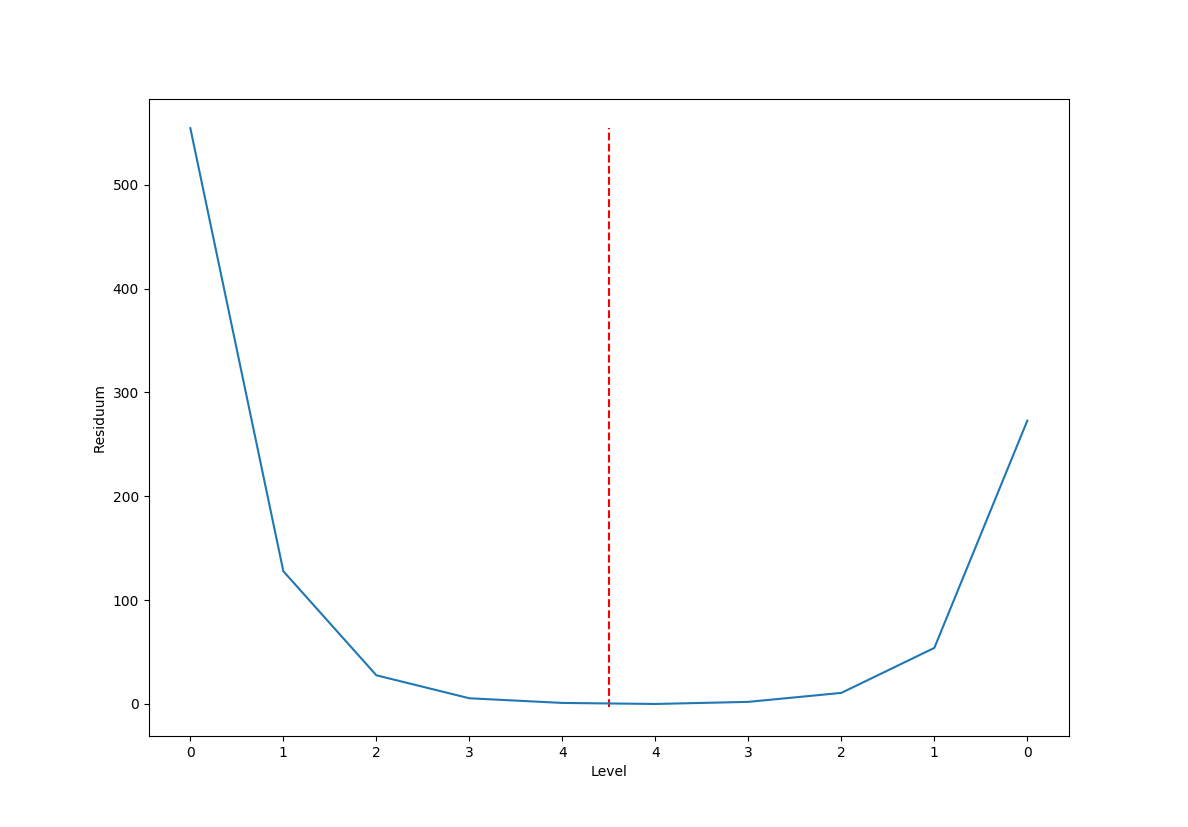
\includegraphics[width=0.9\linewidth, height=7cm]{MG_res_by_level.png}
  \end{center}
\end{frame}

\begin{frame}
  \frametitle{Mehrgitter Konvergenzanalyse}
  \begin{center}
    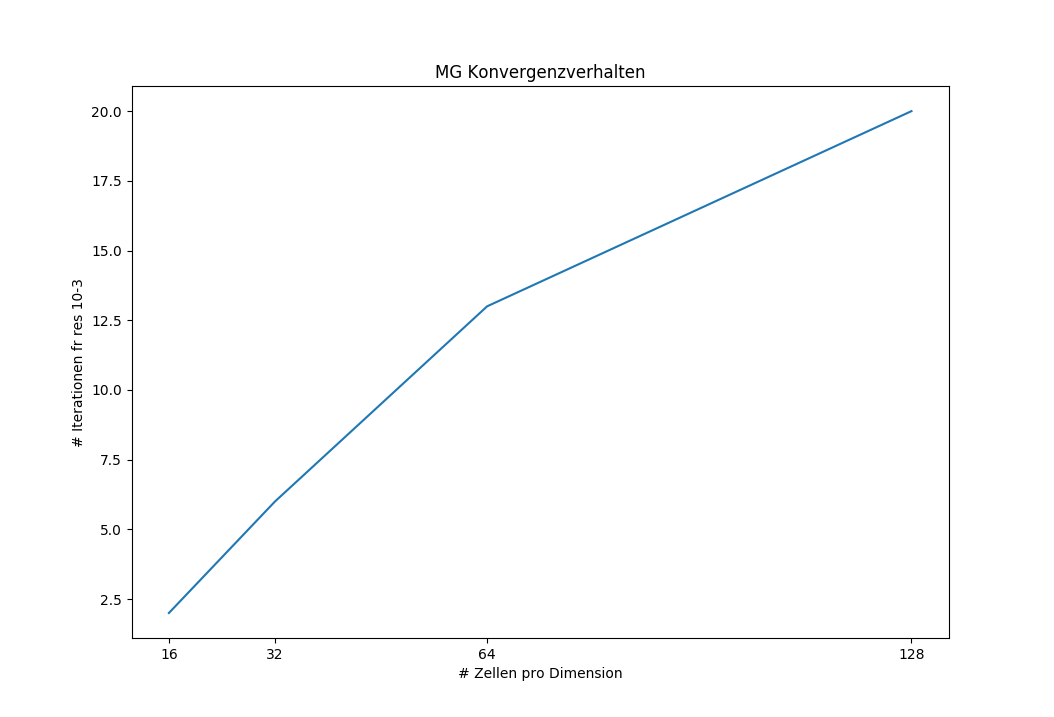
\includegraphics[width=0.9\linewidth, height=7cm]{mg_konvergenzverhalten.png}
  \end{center}
\end{frame}

\begin{frame}
  \frametitle{Vergleich mit SOR}
  \begin{center}
    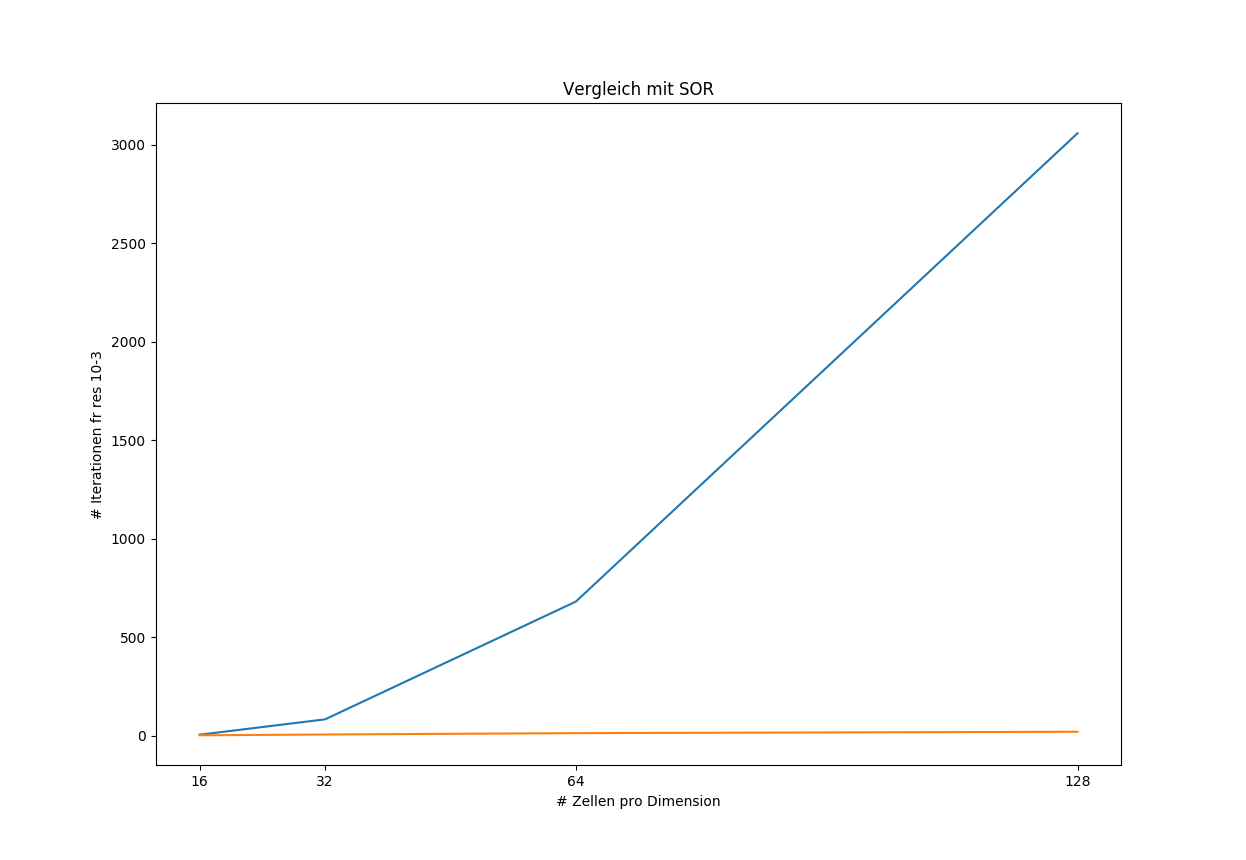
\includegraphics[width=0.9\linewidth, height=7cm]{mg_vs_sor.png}
  \end{center}
\end{frame}


\begin{frame}
\begin{center}
 \Large konjugierte Gradienten Verfahren
 \end{center}
\end{frame}

\section{Verfahren der konjugierten Gradienten}
\begin{frame}
  \begin{algorithmic}
    \Function{CG::Cycle}{ p, res, dir}
    \ForAll{ InteriorIterator it }
     \State Ad.\Call{Cell}{it} $\gets$ dir.\Call{dxx}{it} + dir.\Call{dyy}{it};
    \EndFor

    \State res\_old $\gets$ res.\Call{dotProduct}{res}
    \State alpha $\gets $ res\_old / dir.\Call{dotProduct}{Ad}


     \State p $\gets$ p + alpha * dir;
     \State res $\gets$ res - alpha * Ad;


    \State res\_new $\gets$ res.\Call{dotProduct}{ res };
    \State beta = res\_old / res\_new;

    \State dir $\gets$ dir + beta * res;

    \State \Return res\_new;
    \EndFunction
  \end{algorithmic}
\end{frame}



\begin{frame}
\frametitle{Konvergenzverhalten}
\begin{center}
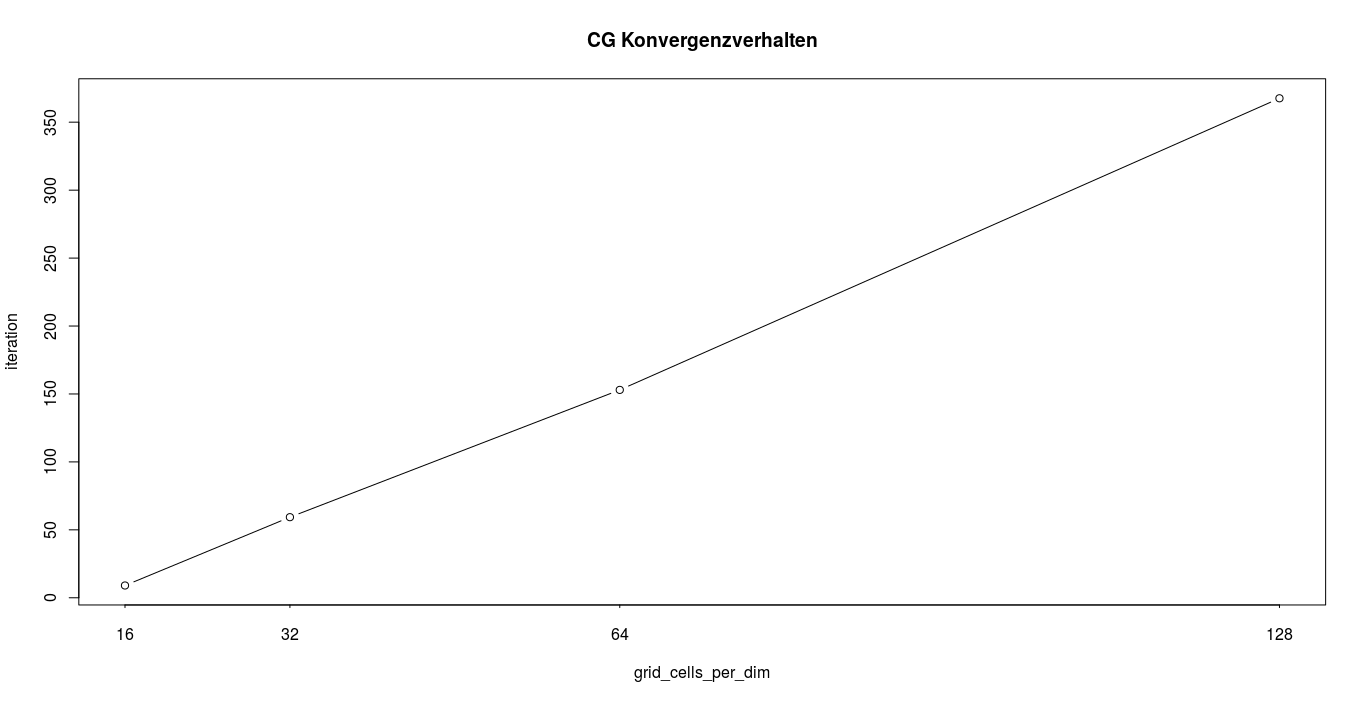
\includegraphics[scale=0.22]{CG_Konvergenzverhalten.png}
\end{center}
\end{frame}


\begin{frame}
\frametitle{Konvergenzverhalten}
\begin{center}
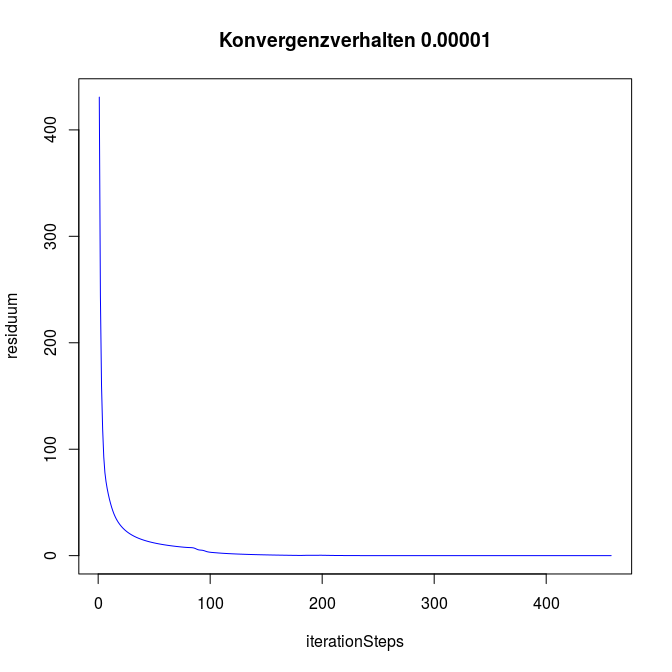
\includegraphics[scale=0.3]{Konvergenz.png}
\end{center}
\end{frame}

\end{document}
